\section{Case1 および Case2 における挙動}
\label{subsec:case12_result}

Case1 および Case2 では，床の沈み込み量が比較的小さく，DS から SS へ移行する瞬間においても自重によって生じる転倒モーメントが小さい条件である．このため，提案手法を適用した場合においても歩行挙動自体に大きな変化は見られなかった （\cref{fig:case1_algo_zmp}, \cref{fig:case2_algo_zmp}）．

実際に，支持脚ロール方向トルクや ZMP の時間履歴を比較すると，従来手法と提案手法の間に顕著な差は確認されず，両者はほぼ同様の挙動を示した．これは，もともと転倒リスクが小さい条件においては，提案手法による補正効果が顕在化しにくいことを示している． 

\begin{figure}[htbp]
  \centering
  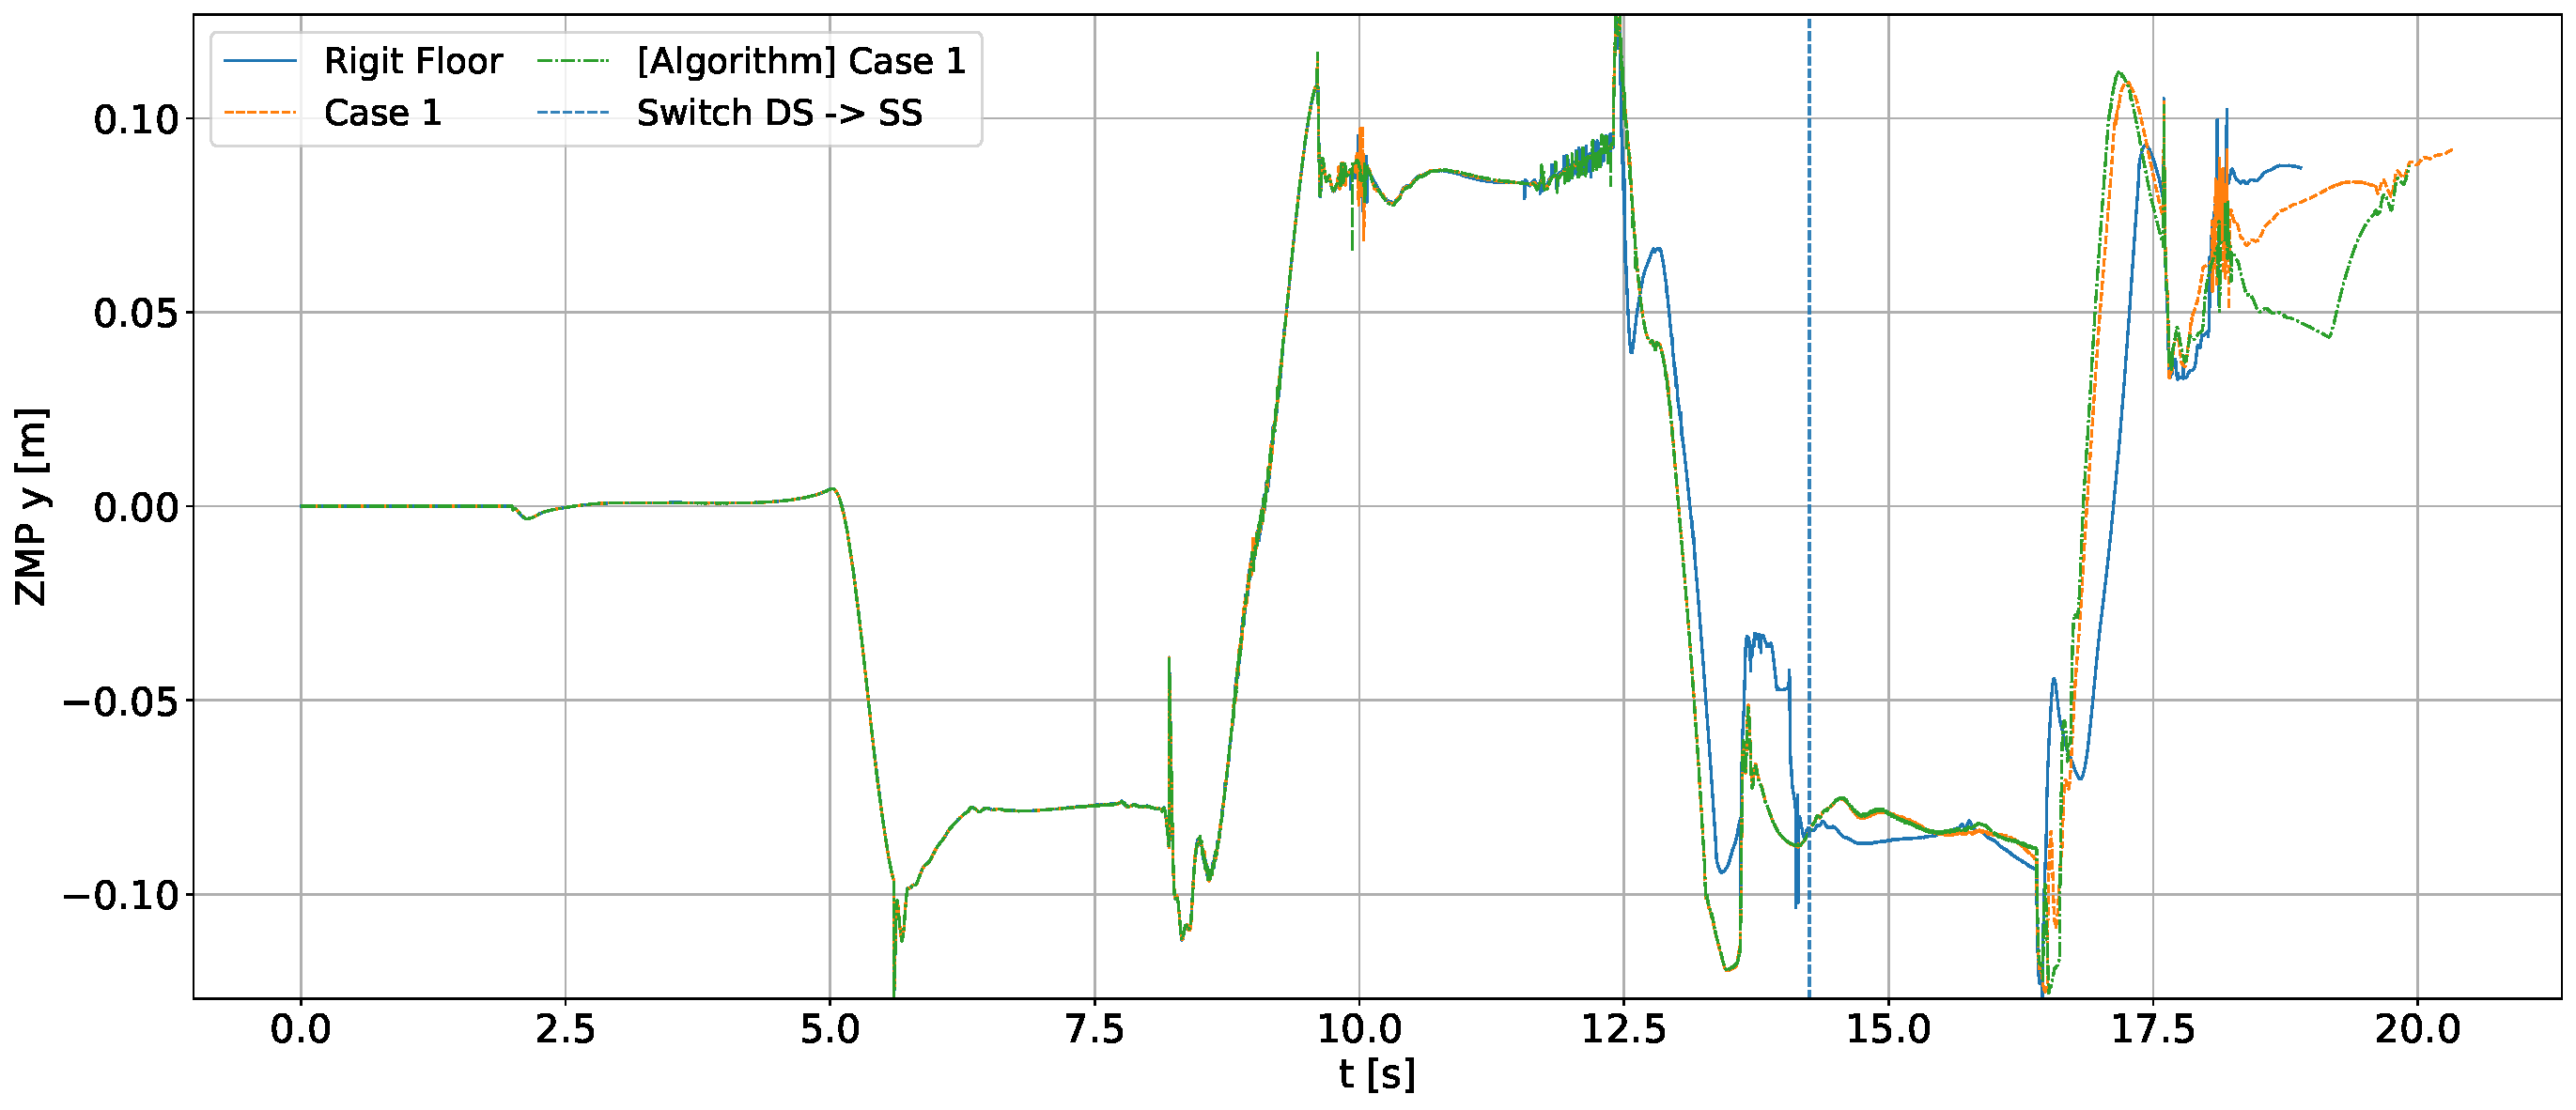
\includegraphics[width=1.0\linewidth]{images/Case1_algo_zmp.pdf}
  \caption{Case1 におけるZMP軌道（提案手法適用時）}
  \label{fig:case1_algo_zmp}
\end{figure}

\begin{figure}[htbp]
  \centering
  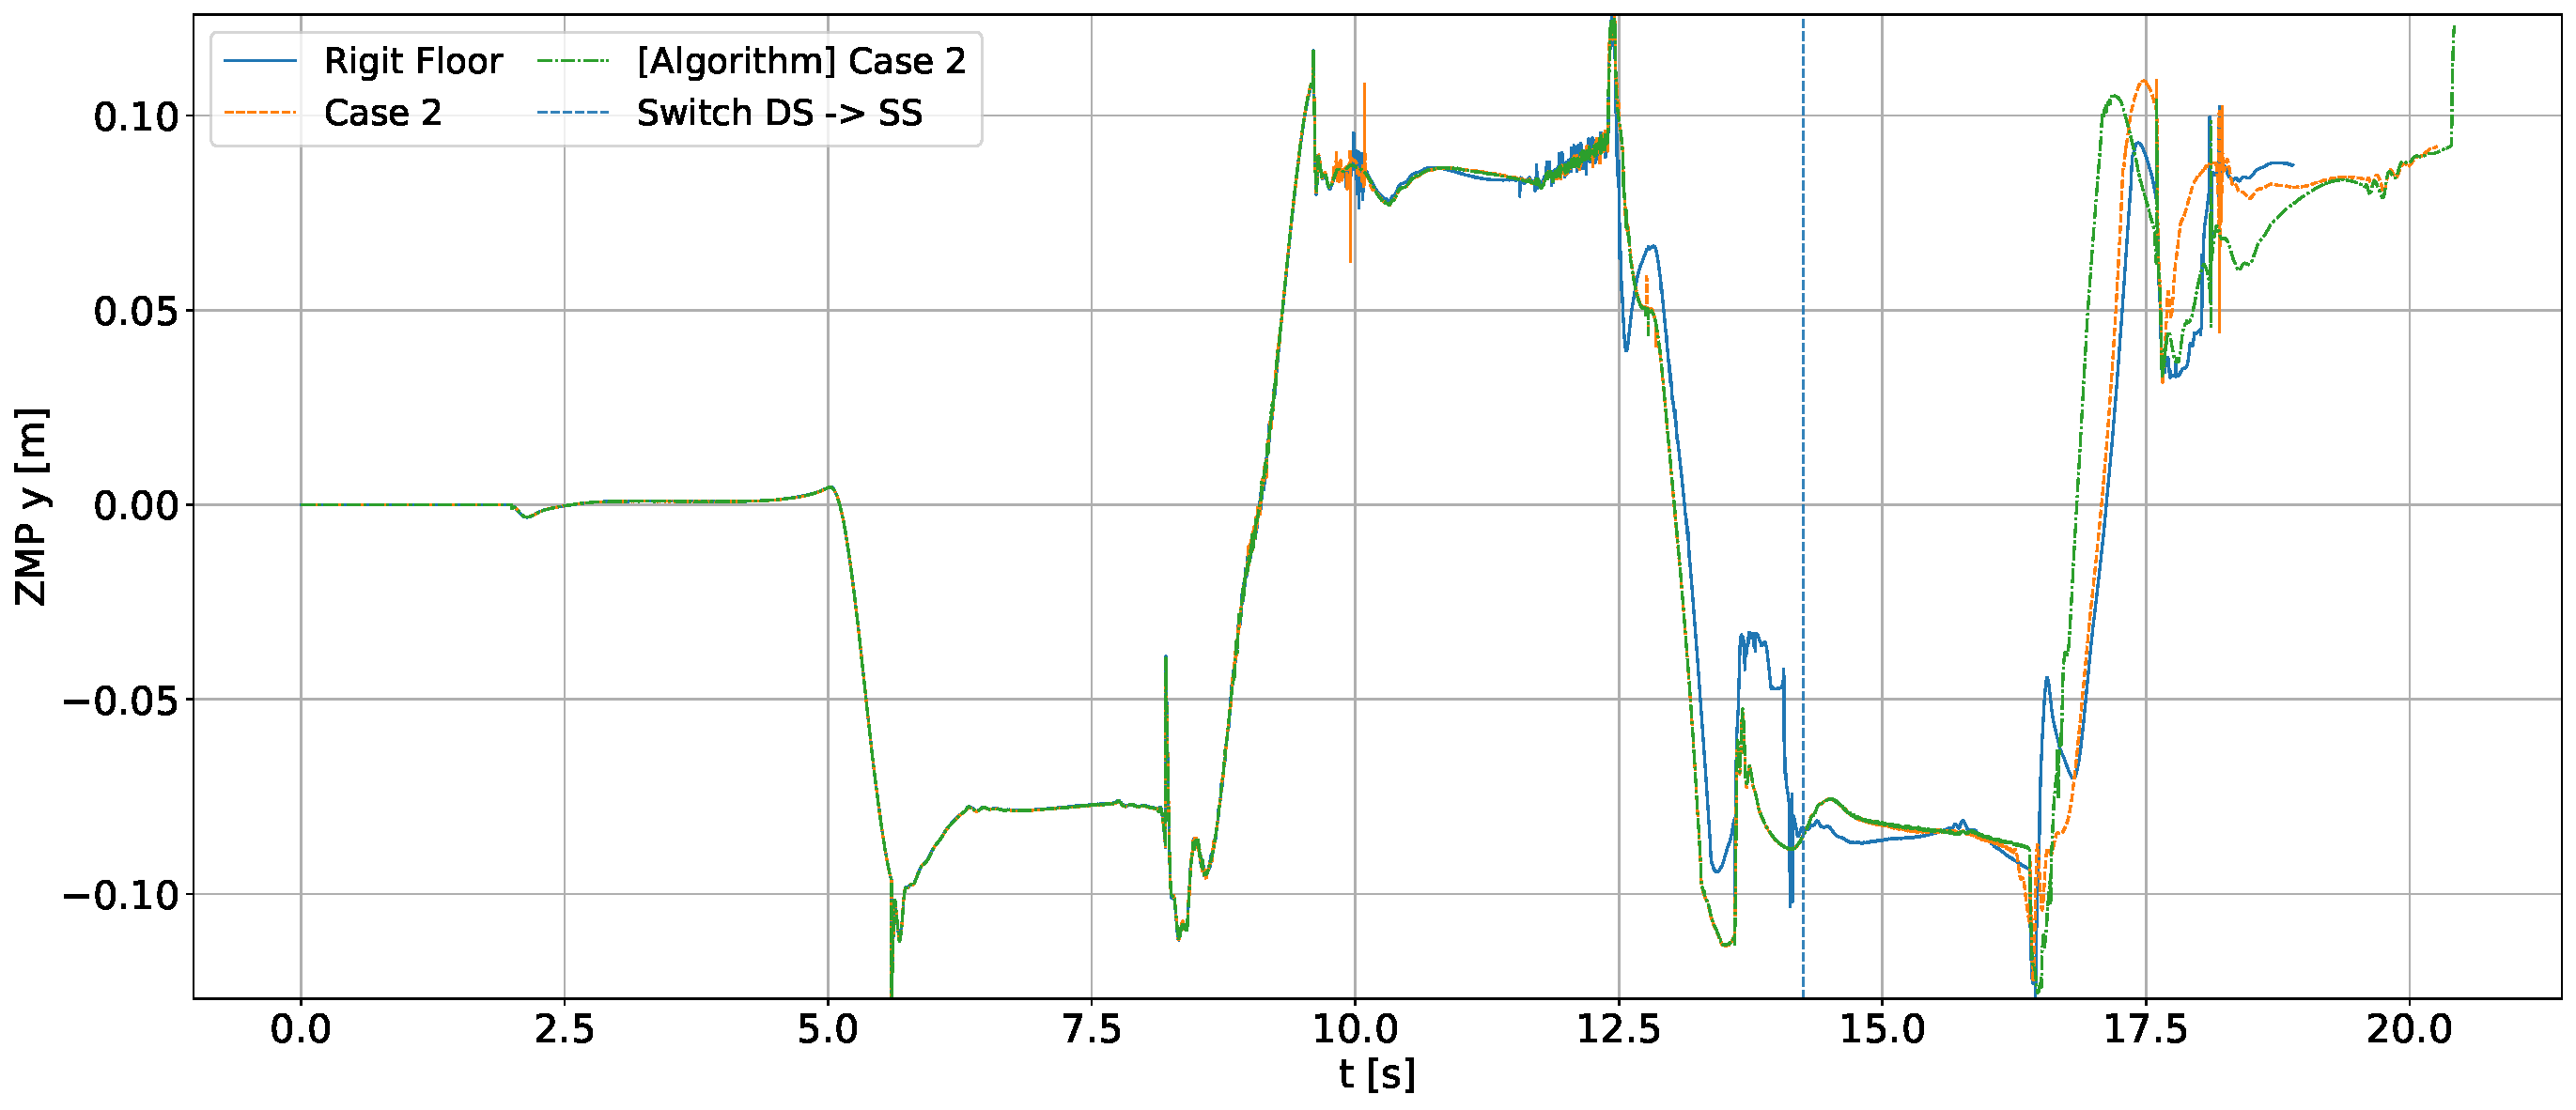
\includegraphics[width=1.0\linewidth]{images/Case2_algo_zmp.pdf}
  \caption{Case2 におけるZMP軌道（提案手法適用時）}
  \label{fig:case2_algo_zmp}
\end{figure}

\clearpage

\section{Case3 における転倒挙動}
\label{subsec:case3_result}

Case3 では，床の沈み込みが急激に生じる条件であり，DS から SS へ移行する際に支持脚に大きな自重モーメントが発生する．この条件においては，提案手法を適用した場合であっても転倒を回避することができなかった．\cref{fig:case3_algo_zmp} を参照しての通り，DS から SS へ移行するよりも前に ZMP が支持脚足裏外側へ発散し，転倒に至る挙動が観測された．

これは，沈み込み速度が極めて大きい場合には，重心高さの調整やトルクの緩和以前に，沈み込みによる体制の不安定化により，転倒方向への倒れ込みが急激に進行してしまうためであると考えられる．この結果は，提案手法がすべての沈み込み条件に対して万能ではないことを示す一方で，適用可能な条件範囲の存在を示唆している．

\begin{figure}[htbp]
  \centering
  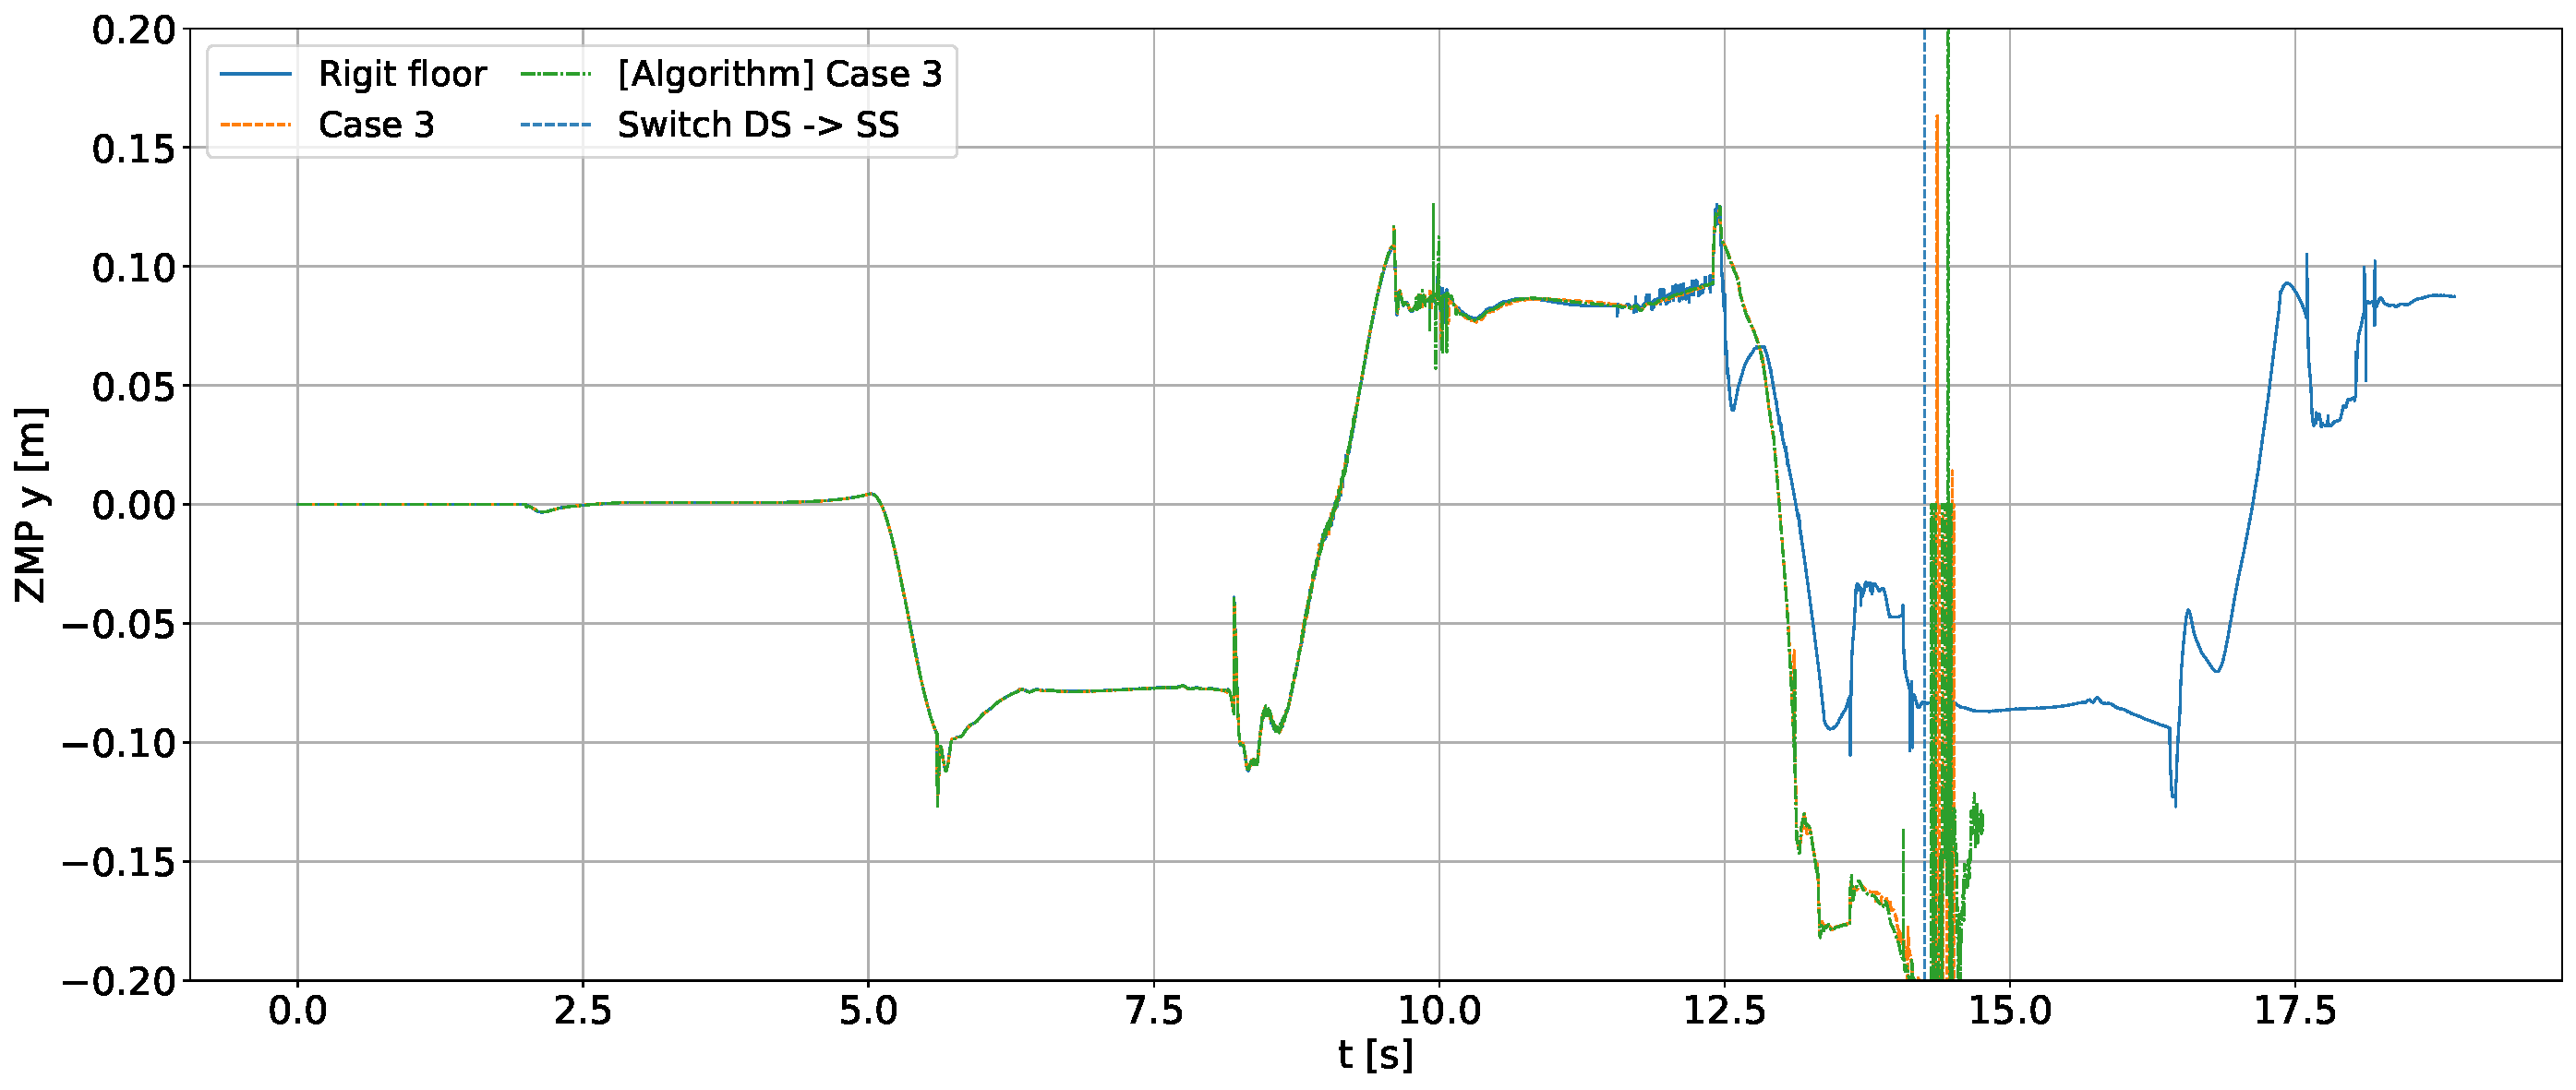
\includegraphics[width=1.0\linewidth]{images/Case3_algo_zmp.pdf}
  \caption{Case3 におけるZMP軌道（提案手法適用時）}
  \label{fig:case3_algo_zmp}
\end{figure}

\section{Case4 における安定歩行の実現と要因分析}
\label{subsec:case4_result}

Case4 では，提案手法を適用することで，従来手法では転倒していた条件においても歩行を継続することが可能となった．以下では，その要因について ZMP，CoM 高さおよび支持脚トルクの観点から順に分析する．

まず，ZMP の時間履歴を比較する．ZMP の軌跡を見ると，DS 期間においては，提案手法適用時においても従来手法と同様に，ZMP が支持脚側の外側境界付近に張り付く挙動が確認された．このことから，DS 期間における ZMP の位置自体には，提案手法による大きな変化は生じていないことが分かる（\cref{fig:case4_algo_zmp}）．

一方で，DS から SS へ切り替わる瞬間の前後の挙動には顕著な差が見られる．従来手法では，SS 移行直後に ZMP が支持多角形外側へ発散し，結果として転倒に至るのに対し，提案手法適用時には，SS 期間においても ZMP が支持脚足裏領域内に留まり，発散することなく安定した挙動を示していることが確認された．この結果は，提案手法によって SS 移行後の不安定化が抑制されていることを示している．

\begin{figure}[htbp]
  \centering
  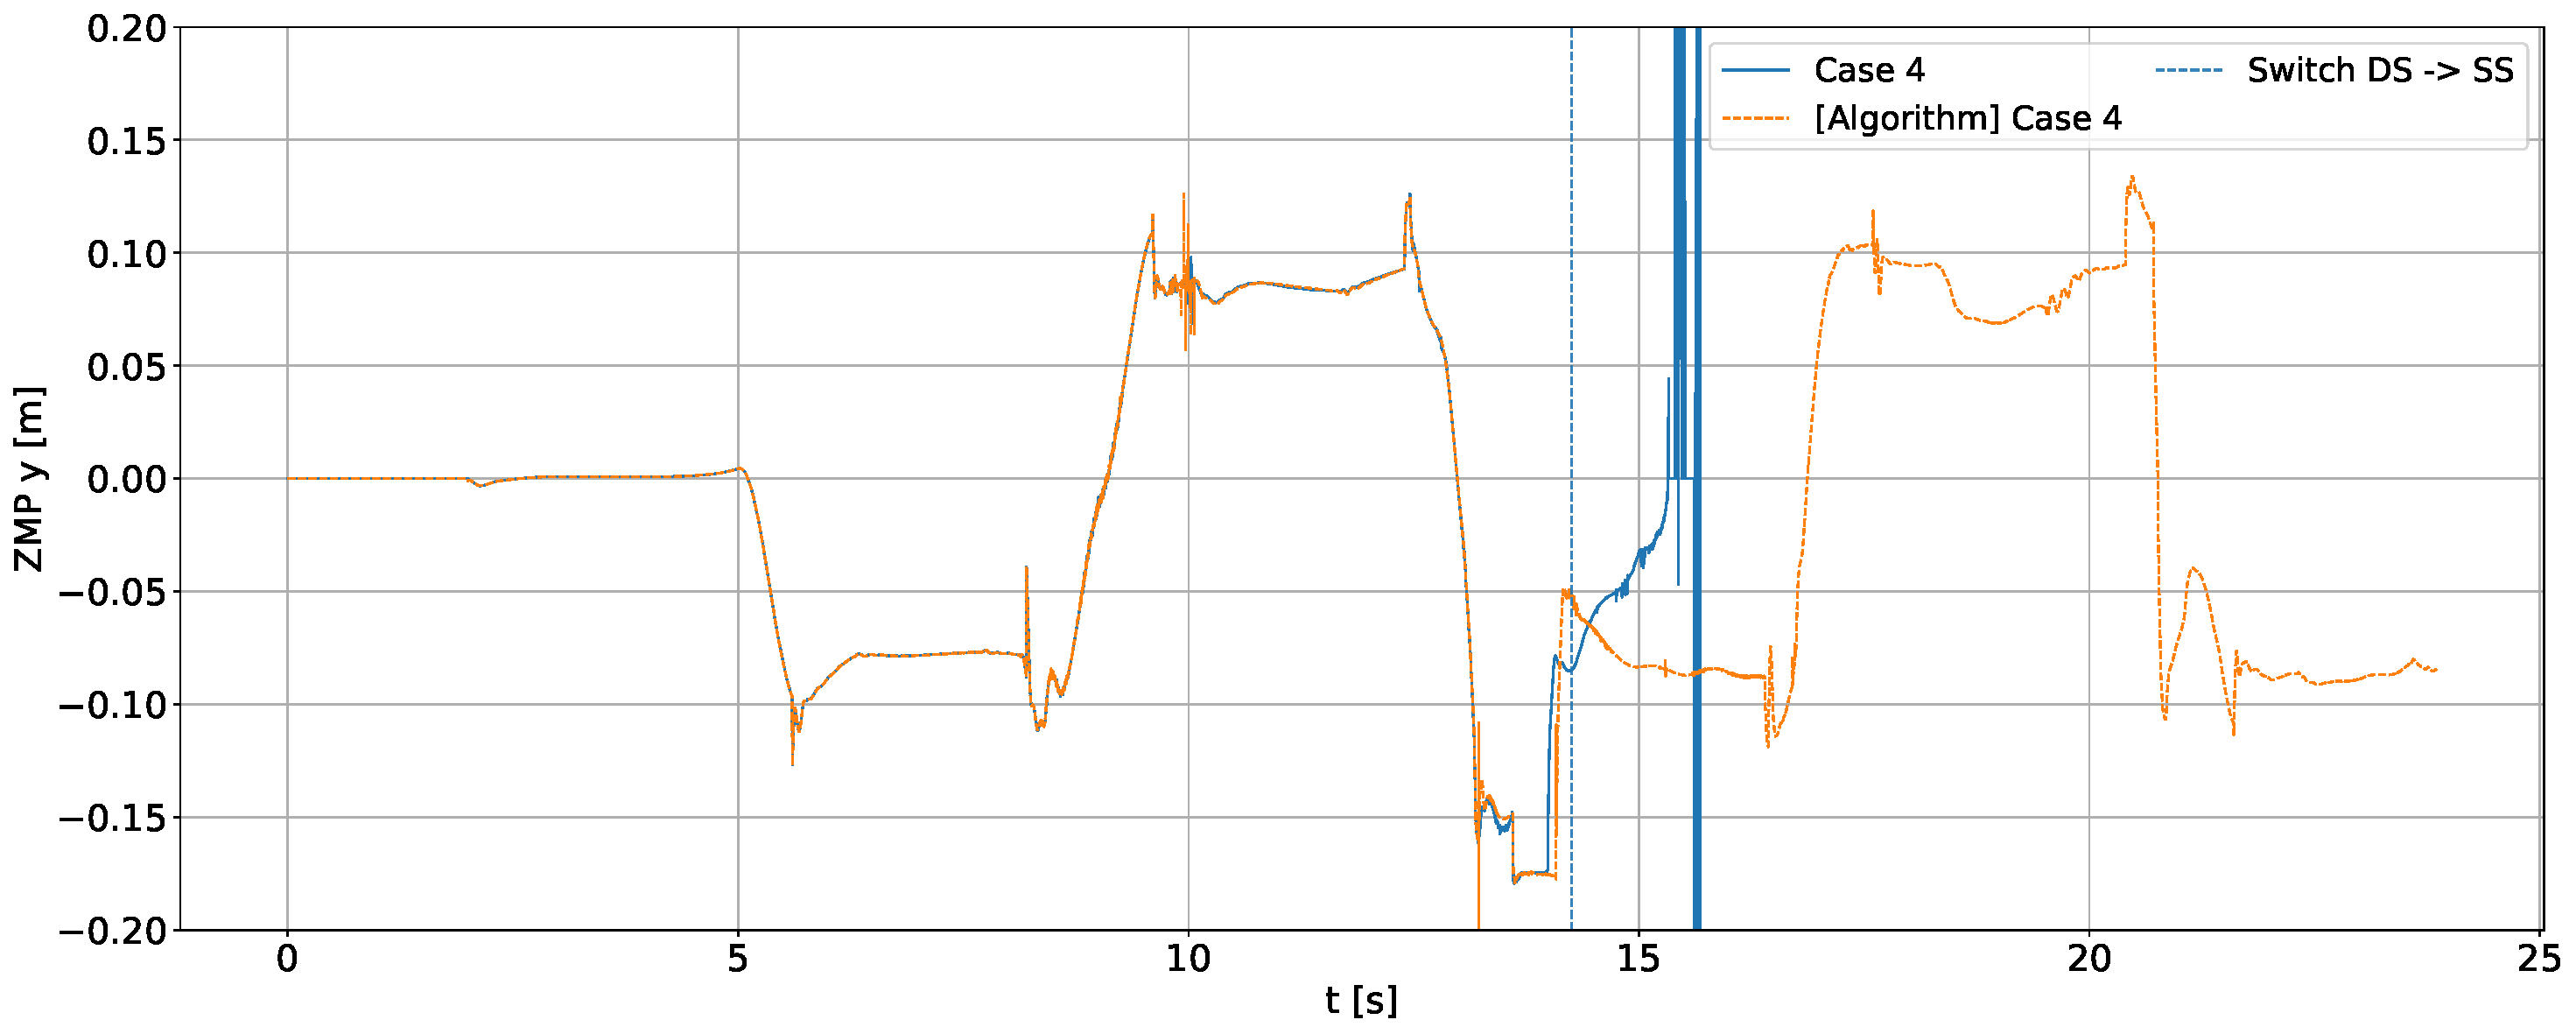
\includegraphics[width=1.0\linewidth]{images/Case4_algo_zmp.pdf}
  \caption{Case4 におけるZMP軌道（提案手法適用時）}
  \label{fig:case4_algo_zmp}
\end{figure}

次に，CoM 高さ $z$ の時間履歴を比較した結果，提案手法適用時には DS から SS へ移行する直前および移行直後において，CoM の $z$ 座標が従来手法と比較して高く保たれていることが確認された（\cref{fig:case4_algo_comz}）．従来手法でも CoM 高さがある程度保証されているのはアドミッタンス制御の影響である．
さらに，支持脚ロール方向トルクの時間履歴を比較すると，DS から SS へ切り替わる瞬間における自重に起因するトルクのピーク値が，提案手法適用時には明確に低減していることが確認された（\cref{fig:case4_algo_torque}）．以上の結果から，CoM 高さを操作することにより足首に作用するロール方向トルクが低減されるという \cref{sec:method_overview} での仮説を支持する結果が得られた．

\begin{figure}[htbp]
  \centering
  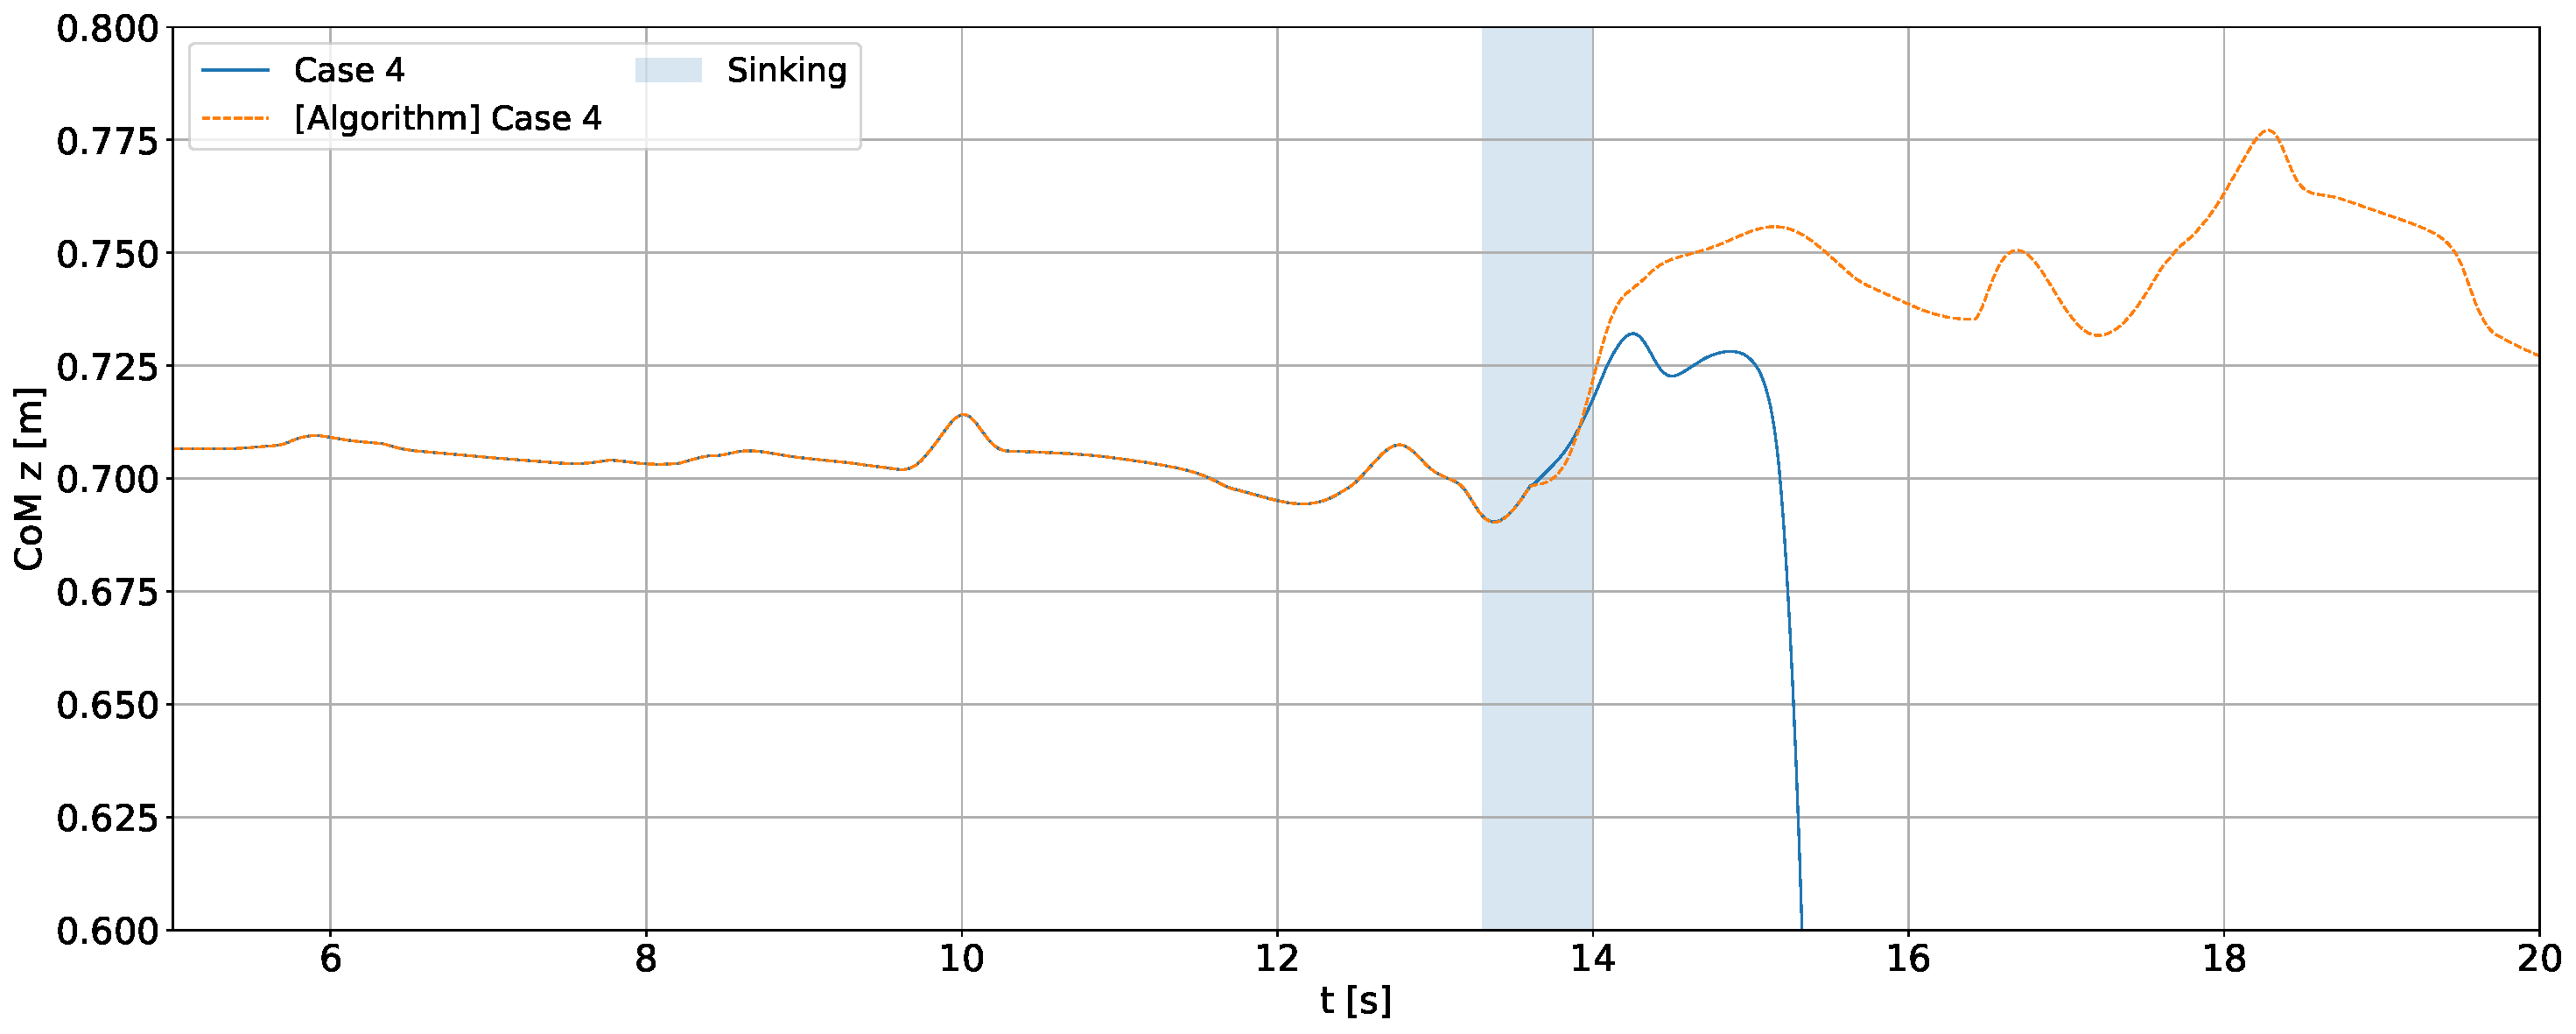
\includegraphics[width=1.0\linewidth]{images/Case4_algo_comz.pdf}
  \caption{Case4 における重心高さの時間履歴比較}
  \label{fig:case4_algo_comz}
\end{figure}

\begin{figure}[htbp]
  \centering
  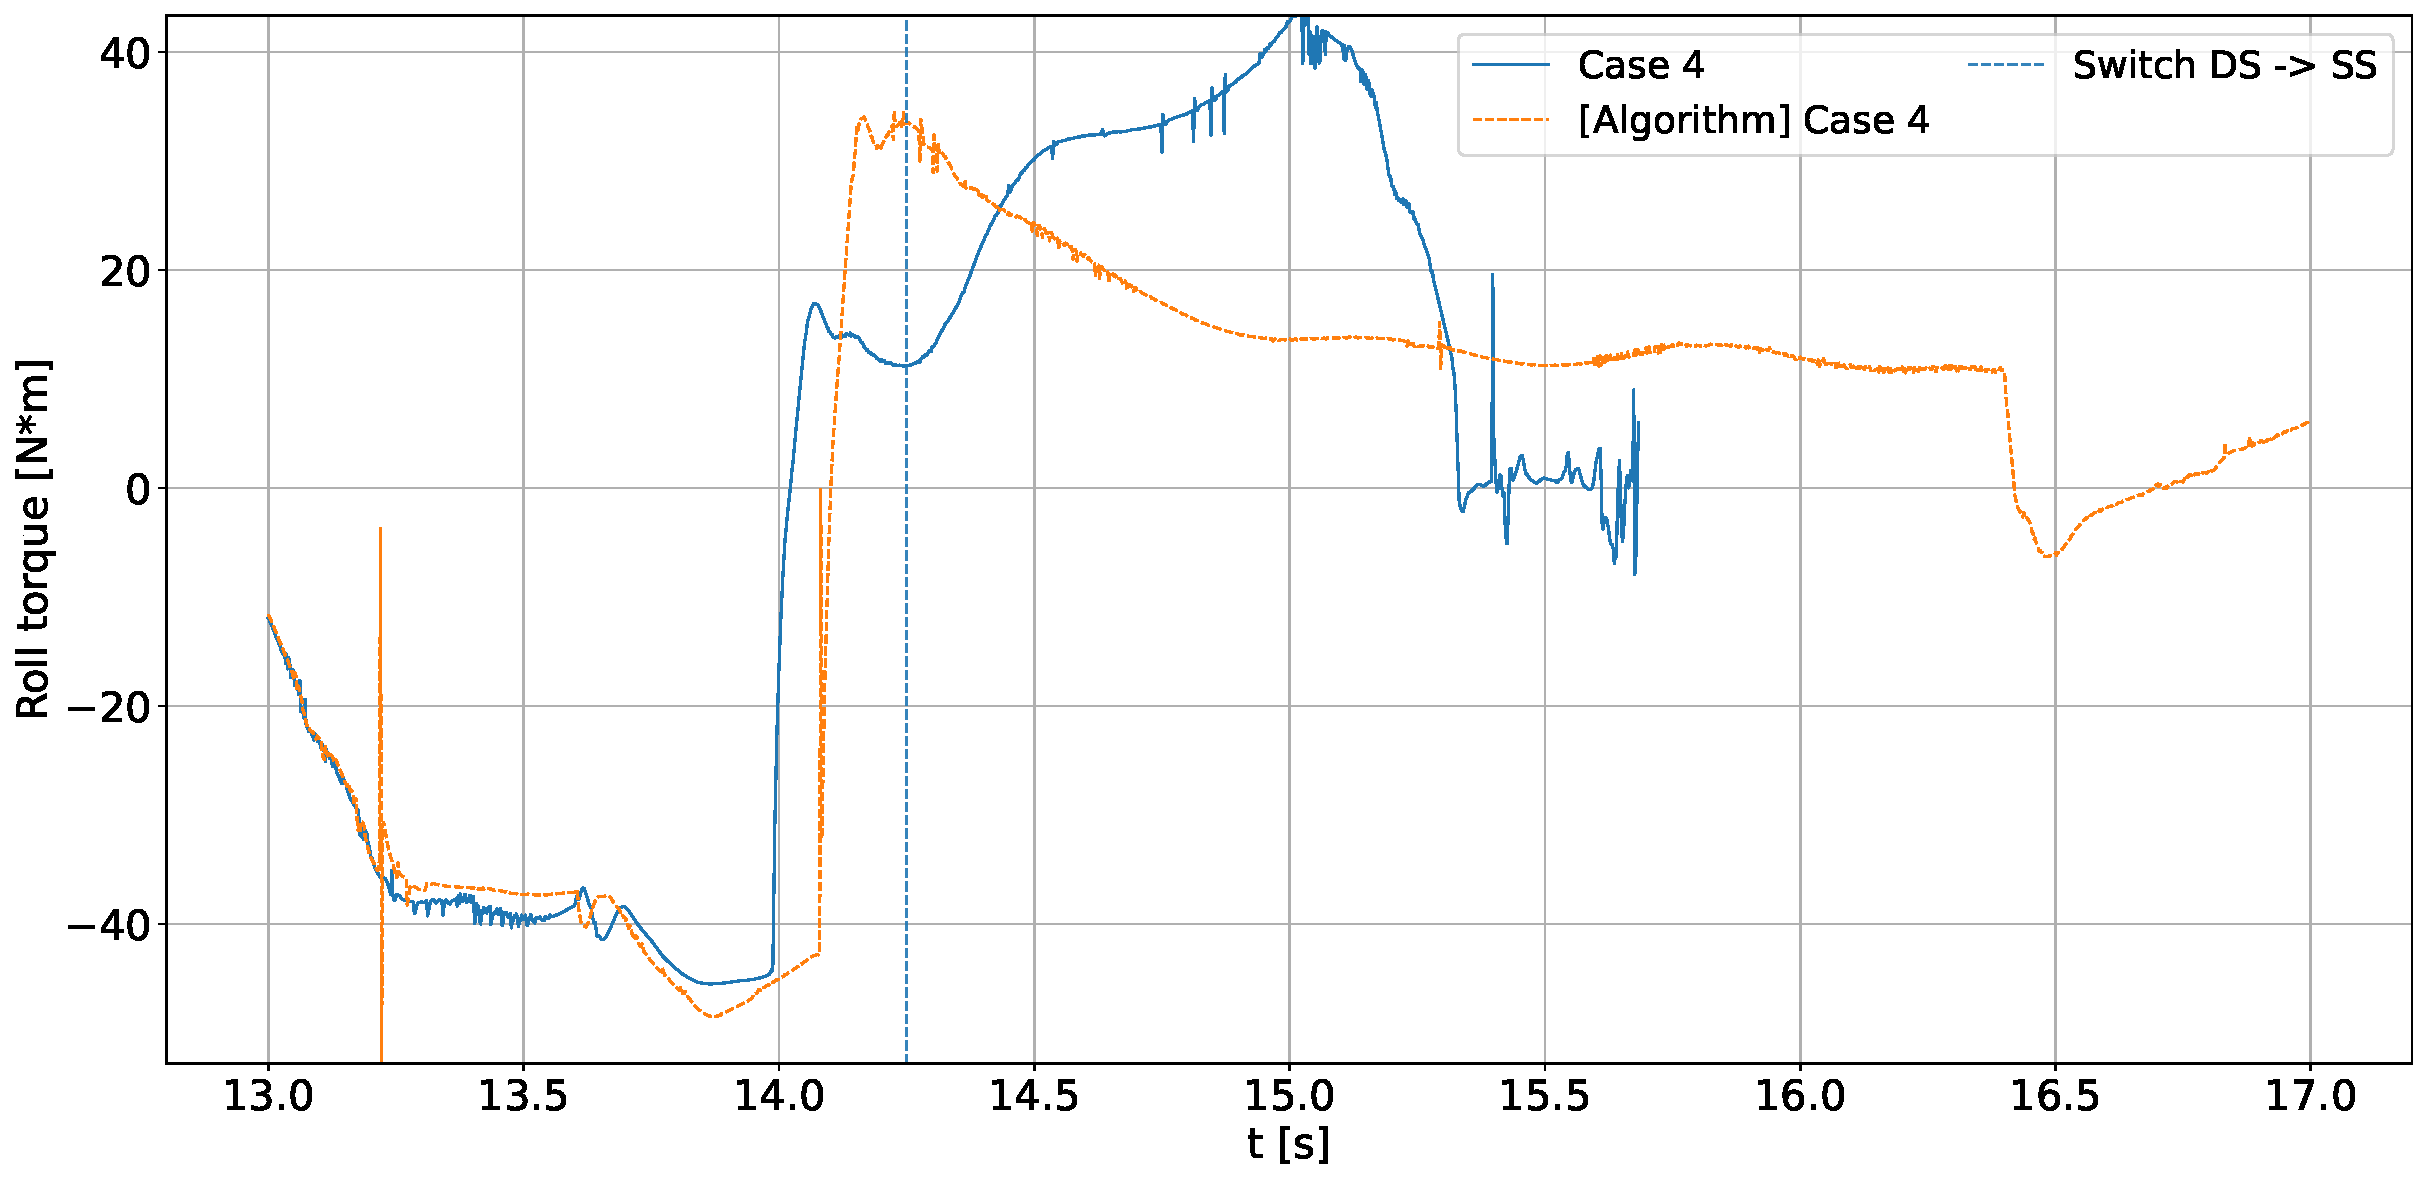
\includegraphics[width=1.0\linewidth]{images/Case4_algo_torque.pdf}
  \caption{Case4 における支持脚ロール方向トルクの時間履歴比較}
  \label{fig:case4_algo_torque}
\end{figure}

